 %--------------------
% Packages
% -------------------
\documentclass[11pt,a4paper]{article}
\usepackage[utf8x]{inputenc}
\usepackage[T1]{fontenc}
\usepackage{tgbonum}
\usepackage{gentium}

\usepackage{multirow}
\usepackage[table]{xcolor}% http://ctan.org/pkg/xcolor
\usepackage{amsmath,amsfonts,amssymb,amsthm}
\usepackage{import}
\usepackage{abstract}
% Algorithm pseudocode
\usepackage{algorithm}
\usepackage[noend]{algpseudocode}

\usepackage{subcaption}
\usepackage{caption}
\usepackage{mathptmx} % Use Times Font
\usepackage[pdftex]{graphicx} % Required for including pictures
\usepackage[english]{babel} 
\usepackage[pdftex,linkcolor=black,pdfborder={0 0 0}]{hyperref} % Format links for pdf
\usepackage{calc} % To reset the counter in the document after title page
\usepackage{enumitem} % Includes lists
\usepackage{xspace}
\frenchspacing % No double spacing between sentences
\linespread{1.5} % Set linespace
\usepackage[a4paper, lmargin=0.1666\paperwidth, rmargin=0.1666\paperwidth, tmargin=0.1111\paperheight, bmargin=0.1111\paperheight]{geometry} %margins
%\usepackage{parskip}

\usepackage[all]{nowidow} % Tries to remove widows
\usepackage[protrusion=true,expansion=true]{microtype} % Improves typography, load after fontpackage is selected

\newtheorem{theorem}{Theorem}
\newtheorem{lemma}{Lemma}
\newtheorem{definition}{Definition}
\newtheorem{corollary}{Corollary}
\newtheorem{proposition}{Proposition}
\newtheorem{problem}{Problem}
\newtheorem{property}{Property}


\newcommand{\learnindex}{\textsf{Learned Index}\xspace}
\newcommand{\btree}{\textsf{B+tree}\xspace}

\newcommand{\fittingtree}{\textsf{FITing-Tree}\xspace}
\newcommand{\conflict}{\textsf{conflict}\xspace}
\usepackage[acronym,toc]{glossaries}


%-----------------------
% Set pdf information and add title, fill in the fields
%-----------------------
\hypersetup{ 	
pdfsubject = {},
pdftitle = {AdaptiveGapsPlacement},
pdfauthor = {Sukphasuth Lipipan}
}



% \makeglossaries
\import{./}{glossaries.tex}
% \newacronym{rmi}{RMI}{Recursive Model Index}
% \newacronym{cdf}{CDF}{Cumulative Distribution Function}
% \newacronym{lipp}{LIPP}{Learned Index Precise Position}
% \newacronym{alex}{ALEX}{Adaptive Learned Index}
% \newacronym{iqr}{IQR}{Interquantile Range}
% \newacronym{tbli}{TBLI}{Tree-Based Learned Index}
% \newacronym{ols}{OLS}{Ordinary Least Square}
% \newacronym{fmcd}{FMCD}{Fastest Minimum Conflict Degree}

%-----------------------
% Begin document
%-----------------------
\begin{document}
% \fontfamily{cmr}\selectfont
\import{./}{titlepage.tex}


\import{./}{declaration.tex}
\clearpage
\listoffigures
\clearpage

\listoftables
\clearpage
\printacronyms


 
\newpage
\tableofcontents


\newpage

{
\centering

\begin{abstract}
\addcontentsline{toc}{section}{Abstract}


The \btree has been the dominant indexing method in database management systems, used by most SQL databases. Recent enhancements take advantage of hardware optimizations such as caching and memory usage. However, the \btree does not make use of existing data patterns and aims to work well for most cases. In contrast, the learned index offers a promising approach to optimizing indexing by leveraging machine learning models to predict the positions of keys and data in the data structure. Initial research on learned index showed significant improvements in search performance and memory consumption compared to traditional \btree. However, the learned index has faced challenges in supporting write operations efficiently. While some approaches have tried to address this issue, they still require overhead for insertion and conflict resolution. This paper proposes a new approach to strategically leaving gaps in the array based on the data distribution and optimizing node creation in the learned index. Results show that our algorithm significantly reduces conflicts and improves read and write operation performance by almost up to $2\times$ compared to the \acrfull{lipp} while also reducing the height of the tree.
\end{abstract}
\newpage
}
\import{./}{introduction.tex}

\import{./}{relatedwork.tex}
\section{Preliminary}
The purpose of this section is to provide an introduction to the concepts and background of our research. By doing so, we hope to provide readers with a better understanding of the context in which our work is situated, and make it easier for them to grasp the key ideas and contributions of our research.

To achieve this goal, we will provide an overview of the field of learned indexes and its relevance to data access and manipulation operations and the model used in Learned Index.

In addition, we will provide background information on the \acrshort{lipp} approach, which is the foundation of our research. We will discuss the structure of \acrshort{lipp}'s node-based index and the components that make it work, such as the gapped array, bitmap index, and linear regression model. We will also highlight some of the key features and benefits of \acrshort{lipp}, as well as its limitations.

\subsection{Linear Regression}
Linear regression is a widely used statistical technique for modeling the relationship between two variables, namely the independent variable, denoted as x, and the dependent variable, denoted as y. The objective of linear regression is to find the best fitting line that represents the relationship between the two variables in the most accurate way possible. The line is represented by the equation $y = mx + c$, where $m$ represents the slope of the line, and $c$ represents the y-intercept.

The main purpose of linear regression is to make predictions based on the relationship between the two variables. In the case of a machine-learned index, linear regression is used to predict the location of the keys in the gapped array. This is done by training a model on a dataset of key and its position. The model learns the relationship between the keys and its location, and can then be used to predict the key's location for new queries.

The process of finding the best fitting line involves minimizing the sum of the squared differences between the actual y-values and the predicted y-values for each data point. This method is known as the method of least squares, and it ensures that the line fits the data points as closely as possible.

One of the reasons why linear regression is used in machine-learned indexes is its simplicity and interpretability. The linear regression model can be easily understood and implemented, and the output can be used to build an index that can efficiently look up rows in the table. Moreover, linear regression can handle large datasets, making it an ideal choice for machine-learned indexes.

In contrast, neural network models can be more complex and computationally expensive, which may cause a large overhead in operations \cite{CasedLearnedIndex}. Therefore, linear regression is a more efficient and practical choice for machine-learned indexes. However, the choice of machine learning algorithm depends on the specific requirements and characteristics of the dataset.

\subsection{Model-Based Insertion}
\begin{figure}
    \centering
    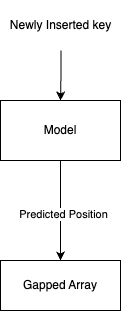
\includegraphics[width=25mm,scale=0.5]{Figures/ModelBasedInsert.png}
    \caption{
     Model-Based Insertion
    }
    \label{fig:model-basedinsertion}
\end{figure}
Model-Based Insertion is essentially an insertion strategy that uses the learned model to determine where newly inserted keys should be placed in the gapped array that constitutes the learned index. The algorithm uses the model to predict the location of the new key, and then places it accordingly to ensure that the learned index can efficiently support insert operations. This is achieved by mapping the keys to the linear regression slope of the model, ensuring that the newly inserted keys fit seamlessly within the existing index structure (Figure \ref{fig:model-basedinsertion}).

\subsection{Learned Index Precise Position} \label{LIPP}
\begin{figure}
    \centering
    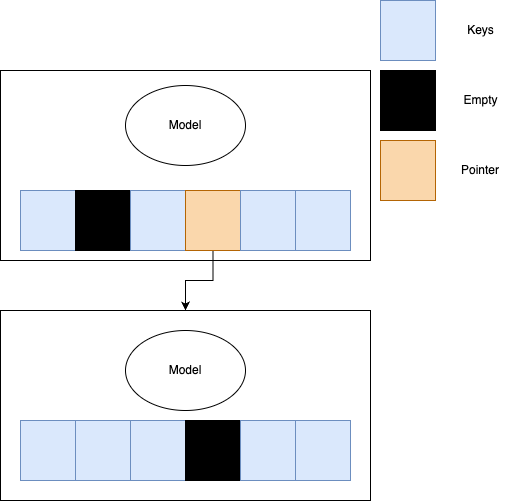
\includegraphics[width=100mm,scale=1]{Figures/LippNode.png}
    \caption{
     \acrshort{lipp} node structure
    }
    \label{fig:lipp-node}
\end{figure}
\acrfull{lipp} adopts a different approach to handling insertion operations compared to other learned indexes such as \acrshort{alex} and PGM \cite{PGM}. Rather than shifting elements or storing them in a temporary buffer to merge later, \acrshort{lipp} employs node creation. This technique involves creating a new node for each new key that is inserted into the index. By creating a new node for each key, \acrshort{lipp} is able to optimize the search operation by ensuring that the output position from the model is exact and precise. This means that \acrshort{lipp} does not need to perform extra searches to locate the key.

However, while \acrshort{lipp}'s node creation approach has several benefits, it also has some limitations. One of the primary concerns with this approach is that it could result in the tree height growing, which could negatively impact the performance of the index. The height of the tree is a critical factor in determining the time complexity of the search operation, and an increase in the height of the tree could result in search operations becoming bound to the height of the tree.

\acrshort{lipp} achieves prediction precision by using a node-based structure that includes a gapped array, a bitmap index, and a linear regression model (Figure \ref{fig:lipp-node}). These components work together to enable accurate and efficient key access.

Furthermore, \acrshort{lipp} introduces the adjustments or branch pruning to reduce the height of the tree. The conditions to trigger the adjustments are (1) current depth after previous adjustments should not be more than $\beta$ times (set to 2 by default) the previous adjustment, and (2) \conflict number should not exceed $\alpha$ (set to 0.1 by default) from the previous adjustments \cite{LIPP}. 

In this research, we aim to build on the foundations of \acrshort{lipp} by developing an algorithm that further enhances its performance. Our algorithm will focus on optimizing performance of \acrshort{lipp}, specifically by improving the gap placement strategy. By doing so, we aim to improve the accuracy and efficiency of key access operations, enabling faster and more reliable data access and manipulation.



\section{Problem Formulation}
\begin{definition}
 Consider an insertion of a new key to the array of a tree node; if the location where the new key should be put in has been occupied, then we say a \emph{conflict} occurs.
\label{def:conflict}
\end{definition}
\begin{definition}
When inserting a new key, we reserve space in the array for keys to guarantee that the data remains sorted, which we call \emph{gaps}.  
\label{def:gap}
\end{definition}

\textbf{Where to place gaps such that the Learned Index is efficient to perform operations like insertion, deletion and query ?}
 
 The \acrfull{lipp} tree structure consists of nodes that hold a gapped array, which contains data, pointers to child nodes, and gaps. Gaps are particularly important for \acrfull{tbli} as they enable support for subsequent key insertions and help reduce the number of conflicts and element shifts \cite{ALEX,PGM,fittingtree,LIPP}. \acrshort{tbli} handle conflicts in different ways, with \acrshort{alex} using the shifting method \cite{ALEX} and \acrshort{lipp} creating a new child node \cite{LIPP}. However, while this method ensures that items remain sorted, it comes with the added computational cost of performing shifts or creating a new node during insertion operations. Shifting requires knowledge of the location of the nearest gap to perform the shift, while creating a new node requires following pointers during range queries.

How can we add gaps to a set of keys with increasing positions $\{x, y\}$ in a way that minimizes conflicts while still maintaining or partially maintaining the monotonicity of the key-position relationship? The number of gaps added should be limited to a maximum value of $M$. The distribution of the density of keys in the set, ${X_1, X_2, \cdots, X_n\ | X \in \mathbb{Q}}$, is represented by $Pr[a \leq X_n \leq b]$. The number of gaps inserted between key $X_i$ and $X_{i+1}$ is $m$, and the total number of gaps in the gapped array should not exceed $M$ (i.e., $\sum_{X_1}^{X_n}{m} \leq M$).

One of the main challenges in optimizing the performance of learned indexes is handling dynamic data. When new data is inserted into the data structure, it may follow a different distribution than the existing keys, making it difficult to determine where to insert gaps to minimize conflicts. However, if the newly inserted data follows the same distribution as the existing keys \textbf{static}, the problem becomes simpler to handle. In this case, we can focus on identifying places where the key density is highest and insert gaps accordingly. By doing so, we can reduce the number of conflicts and avoid the need to create new nodes.

On the other hand, for \textbf{dynamic} data, where the distribution of inserted keys may change over time, it is much harder to tackle the problem of minimizing conflicts. In this case, we need to be able to detect slowly changing distributions and adjust the placement of gaps accordingly. This can be achieved by monitoring the distribution of inserted keys and identifying areas where the density has shifted. Once these areas have been identified, we can insert gaps to reduce the number of conflicts.

Reducing the number of conflicts in each node is crucial to ensuring optimal performance of learned indexes. When conflicts occur, we may need to perform extra computations like creating new nodes, which can lead to a larger tree and poor lookup times. Therefore, by minimizing the number of conflicts, we can avoid these extra computations and keep the tree size manageable. Ultimately, this leads to faster lookup times and more efficient use of resources.

Furthermore, expanding gapped arrays and inserting gaps between keys can be a costly operation in terms of retraining the machine learning models used in the indexes. In order to learn the new positions of the keys after gaps have been inserted, the models need to be retrained. However, the amount of time required to retrain the models can vary depending on the complexity of the model used \cite{CasedLearnedIndex}. For instance, a simple linear regression model is used, the retraining process should be fast, as the model only contains multiplications \cite{CasedLearnedIndex,ALEX,LIPP}. However, more complex models, such as neural networks, may take longer to train on larger datasets, making it impractical to retrain the models frequently \cite{CasedLearnedIndex}. Therefore, finding a balance between the complexity of the model and the time required to retrain it is essential when optimizing mutable learned indexes.



\import{./}{methodology.tex}
% \import{./}{preliminaryresult.tex}



\section{Histogram}
\subsection{Implementation Details}
\subsubsection{Insertion}
\begin{algorithm}
\caption{Histogram Insertion}
\begin{algorithmic}[1]

\Procedure{Insertion Procedure}{}
% \State $\texttt{MAX_DEPTH} \gets 128$

\EndProcedure
\end{algorithmic}
\end{algorithm}




The strategy we employ for the insertion of histograms is very similar to that of the baseline strategy. However, there are some noteworthy differences in the way we rebuild nodes. Rather than relying on the traditional methods, we use a histogram approach to obtain an approximate distribution of the data. This allows us to generate keys, denoted by $x$, and their corresponding positions or labels, denoted by $y$.

To further refine the model, we use Ordinary Least Square (OLS) to obtain the slope and y-intercept for linear regression. This aids in the accurate identification of conflicts within the data. The rebuilding process occurs when a new node has a depth that is at least twice that of the previous node, in a similar fashion to the baseline strategy.

In cases where conflicting elements arise, a new node is created to ensure the integrity of the data. However, the creation of new nodes comes with an additional computation, which slows down the insertion time. This is because the model needs to be trained to accommodate these conflicting keys and accurately insert them into the gapped array.

Overall, the insertion strategy for histograms relies on a combination of techniques such as the use of OLS and histogram analysis to ensure that the data is accurately represented and conflicts are resolved promptly. While it may result in slightly slower insertion times, the benefits of a more accurate representation of the data outweigh the costs.

\subsubsection{Query}
\begin{algorithm}
\caption{Histogram Query}
\begin{algorithmic}[1]

\Procedure{Query Procedure}{}
% \State $\texttt{MAX_DEPTH} \gets 128$

\EndProcedure
\end{algorithmic}
\end{algorithm}

To perform a search operation in \learnindex, the algorithm starts at the root node of the tree and traverses down to the leaf nodes to find the data. One of the advantages of \learnindex is that it uses a model-based insertion technique, which allows it to perform search operations efficiently. When there is a conflict during insertion, \learnindex creates a new child node rather than shifting the keys to the closest gaps. This ensures that there are no misplacement in the index, which can slow down search operations by making performing search after traversing down the tree.

The search algorithm in \learnindex starts by pushing the root node into the stack. Using the current node's linear regression model, the algorithm predicts the position of the keys it is searching for. It then checks if the predicted position is a child or a key. If the predicted position is a child, the algorithm pushes the child node onto the stack and continues the search. If the predicted position is a key, the algorithm returns the key.

The child node continues to be pushed onto the stack until the algorithm reaches the node that contains the key it is searching for. This process allows for efficient search operations, as the algorithm only explores the parts of the tree that contain the key it is searching for.

\subsubsection{Deletion}

\begin{algorithm}
\caption{Histogram Delete}
\begin{algorithmic}[1]

\Procedure{Deletion Procedure}{}
% \State $\texttt{MAX_DEPTH} \gets 128$

\EndProcedure
\end{algorithmic}
\end{algorithm}
Deletion is an essential operation for any data structure that stores data, and \learnindex is no exception. Deletion in \learnindex follows a similar strategy as search, where the algorithm has to traverse down the tree until reaching the node where the key is located. Once the node is found, the key can be removed from the tree.
However, there is a critical difference between deletion and search in \learnindex. During deletion, the algorithm must also free up space in the gapped array, and also update the bitmap index that this position contains a gap instead of a key.

To perform the deletion, the algorithm starts at the root node and uses the same model-based approach to predict the position of the key. As the algorithm descends the tree, it checks each node's bitmap to determine whether the key is present in that node. Once the node containing the key is found, the key is deleted, and the algorithm updates the bitmap that stores it in the current node.


\subsubsection{Range Query}
\begin{algorithm}
\caption{Histogram Range Query}
\begin{algorithmic}[1]

\Procedure{Range Query Procedure}{}
% \State $\texttt{MAX_DEPTH} \gets 128$

\EndProcedure
\end{algorithmic}
\end{algorithm}

Range queries are an essential operation in \learnindex, particularly when dealing with sorted collections of keys. Such queries involve searching for a range of keys within a given dataset and are commonly used in a wide range of applications, including databases, search engines, and information retrieval systems.

One of the advantages of using a sorted dataset is that it makes range queries relatively easy to perform. By searching for the first key in the range and then iterating through the data structure to collect all keys until the end key is reached, the algorithm can efficiently retrieve all of the data within the specified range.


\subsubsection{Adjustments}

\begin{algorithm}
\caption{Histogram Gap Distribution}
\begin{algorithmic}[1]
\Procedure{Histogram Distribute}{}

\EndProcedure
\end{algorithmic}
\end{algorithm}
The strategy we employ to make adjustments to the \learnindex structure utilizes the same condition as \acrshort{lipp}. Prior to making any adjustments, our algorithm traverses the data structure and collects the keys that will be involved in the adjustments. We then create a new node to store these keys. 

However, our approach differs in the way we analyze the collected data. Rather than using \acrfull{fmcd}\cite{LIPP}, we use a histogram to examine the distribution of the data and select a bin width based on the characteristics of the collected data.  By doing so, we are able to make more informed decisions about the optimal size of the bin width, which can ultimately lead to more efficient and effective adjustments to the \learnindex.




\subsection{Theoretical Analysis}
When inserting a node into a gapped array, the algorithm must traverse down the tree until it finds an empty gap to fill. This process takes $O(\log N)$ time.

However, the linear regression model used to predict the position of keys is much more efficient, taking only $O(1)$ time due to its reliance on simple multiplication operations. Additionally, when a new node is inserted into the tree, the histogram in each node must be updated to reflect the new frequency of data points.

To accomplish this, we use an array of frequencies and calculate the bin index using the formula $bin\_index = floor((data\_point - min\_value) / bin\_width)$. The calculation of the bin index for a single data point takes only $O(1)$ time due to the simplicity of the arithmetic operations and the use of the floor function. However, insertions need to be readjusted when the condition is met, similar to the \acrshort{lipp} index, which will cost $O(N\log N)$ where N is the number of keys in the tree. In adjustments, gap redistribution is required and retrained the model to get the accurate prediction of keys and location. However, the adjustments does not occur every time we traverse down the tree path. In this case, we can amortize the cost such that we save $\log N$ credit every time we pass a path which makes the insertion costs similar to the baseline which is $O(\log^2 N)$

However, the time complexity for updating the histogram frequency with bin width using an array varies depending on the number of data points that map to the same bin. In the best case, the time complexity for updating the frequency is $O(1)$, as updating an element in an array takes constant time. However, in the worst case, the time complexity for accessing the frequency element is $O(\epsilon)$, where $\epsilon$ is the number of data points that map to the same bin. This is because computing the index to access the array element can require linear time.

Therefore, the efficiency of updating the histogram frequency in each node during the insertion process can vary greatly depending on the number of data points that map to each bin. However, the overall time complexity of inserting a new node into the gapped array is dominated by the traversal down the tree, which takes $O(\log N)$ time.

However, deleting a key in the \learnindex algorithm involves more than just traversing down the tree. Once the key is located, the algorithm needs to perform deletion and free the memory in the gapped array that was allocated for the key being deleted. This can be a more complex process than insertion, which only involves finding an empty gap in the gapped array and filling it with a new key.

Similar to insertion, when deleting a key, the algorithm must traverse down the tree until it reaches the appropriate node. This process takes $O(\log N)$ time, where $N$ is the number of elements in the tree. Once the node is reached, the algorithm must search for the key to be deleted. If the key is found, the algorithm must then perform deletion and free up the memory in the gapped array for future key insertion. In addition, it takes the same time complexity to update the histogram.

Querying a key in the \learnindex algorithm involves traversing down the tree until the model predicts that the key is located at the current node. This process takes $O(\log N)$ time, where $N$ is the tree's height. Once the key is found, the algorithm returns its position in the gapped array.

The time complexity for querying a key in the \learnindex algorithm is dominated by the traversal down the tree. Since the linear regression model used by the algorithm can accurately predict the position of keys, the search process is generally efficient and does not require additional time complexity.

In summary, the \learnindex algorithm is designed to provide efficient querying capabilities with time complexity of $O(\log N)$, where $N$ is the number of elements. 






\section{Partial Sorted Insert Strategy}
\subsection{Implementation Details}

\subsubsection{Insertion}
When it comes to inserting a new key in the partially sorted gapped array of the \acrshort{lipp} index, the process differs from that of a fully sorted array. Instead of creating a new node in the tree for the key, the algorithm must search for the next available gap within the specified limit to insert the new key. This approach is designed to reduce the memory overhead of the \learnindex data structure, as it eliminates the need to create new nodes for every new key.

Specifically, the algorithm traverses down the tree until it reaches a node containing a key that is within the predicted position of the new key. Once such a node is found, the algorithm scans forward within the array for the next available gap to insert the new key. This process ensures that the new key is inserted in the correct position in the partially sorted array, without requiring the creation of new nodes in the tree.

However, this approach does have a potential downside in terms of computational overhead. Since the partially sorted array is not fully ordered, the algorithm may need to search further than it would in a fully sorted array to find an available gap to insert the key. This extra search can add additional computational complexity to the insertion process, as the algorithm must spend more time searching for an available gap in the array.

To handle \conflict, partially sorted \learnindex needs to iterate $\epsilon$ spaces after predicted position to collect all the partially sorted keys. This process can be time-consuming, especially if the data set is large. In some cases, the algorithm may need to rebuild the whole node entirely to properly sort the partially sorted keys.

A specific example of this can be seen in the context of a gapped array. When the predicted position contains a partially sorted keys, this requires the algorithm to recursive rebuild of both keys. In such cases, the algorithm needs to iterate through the gapped array to collect all the partially sorted keys that may be located $\epsilon$ distance away from the predicted position.

Moreover, rebuilding the gapped array becomes necessary if the predicted position is itself a partially sorted key. In this scenario, a recursive rebuilding process must be undertaken to ensure that the gapped array is correctly sorted, which will also affect the running time of this algorithm.

As mentioned earlier, one approach to handling conflicts in a gapped array data structure is to use a recursive rebuilding approach. However, an alternative approach is to use the percentage of partially sorted keys to determine whether to rebuild the whole node.

This approach takes advantage of the fact that when a high percentage of the keys in a gapped array is partially sorted, it may be more efficient to rebuild the whole node rather than to attempt to rebuild when the \conflict happens. If the number of partially sorted keys is more than $\frac{1}{2}$ of the number of gapped array lengths, then rebuilding the whole node should be considered.

However, it is essential to note that this approach has limitations and may not always be the most efficient way to handle conflicts in a gapped array. It is also essential to consider other factors, such as the size of the data set and the computational resources available.

In this particular work, we will only be tested on the recursive rebuilding approach. This decision was likely made to simplify the testing process and to provide a clear comparison between baseline and partially sorted gapped array. 


\subsubsection{Query}
When it comes to querying a key in the partially sorted gapped array of the \learnindex algorithm, the process is similar to that of insertion. Like insertion, the algorithm must traverse down the tree until it reaches a node containing a key that is within the predicted position of the queried key. If the key in the node is not the same as the queried key, the algorithm must then scan forward within the array up to the specified limit.

This approach efficiently locates the queried key within the partially sorted array while minimizing the memory overhead of the \learnindex data structure. By accurately predicting the position of the queried key using the linear regression model, the algorithm can quickly navigate the gapped array and locate the keys within the partially sorted limit.

However, scanning forward in the array can potentially add computational complexity to the querying process, mainly if the limit specified is far from the predicted position of the queried key. The algorithm must search through the array to find the next available gap within the limit, which can result in additional computational overhead. 


\subsubsection{Deletion}
When it comes to deletion in a data structure such as a \learnindex, the process typically involves searching for specific keys that need removal. However, in the case of a partially sorted gapped array structure, this search process can be more complex, as the keys are not necessarily contiguous and may be spread out over multiple sections of the array.

To perform deletion efficiently in a partially sorted gapped array, the \learnindex algorithm must continue searching for the target keys beyond the predicted location. This typically involves searching until the $\epsilon$ partial sorted limit, where $\epsilon$ is the number of empty spaces after the predicted position the keys can be inserted into.

By continuing the search process this way, the \learnindex can ensure that it locates all of the relevant keys for deletion, regardless of their position within the array. This can be a highly efficient method for performing deletions in large datasets, as it avoids the need for costly full scans of the entire array and instead focuses on the relevant sections of the data structure.
\subsubsection{Range Query}
Typically, when performing a range query on a partially sorted gapped array, the algorithm will search for the first key within the specified range and then iterate through the array, collecting all keys until it reaches the end key. However, even after reaching the end key, there may still be additional keys that fall within the specified range but are located in the $\epsilon$ spaces beyond the end key.

The algorithm must continue searching beyond the end key, ensuring that all relevant keys are included in the range query, considering these additional $\epsilon$ spaces. By doing so, the algorithm can identify any keys not included in the initial search but are still within the specified range, providing a comprehensive and accurate result set.


\subsubsection{Adjustments}
When it comes to working with partially sorted items, several challenges can arise. One of the most significant is that the items are not sorted, and the keys may not follow a consistent, monotonically increasing pattern. This can make it difficult for models to accurately predict the partially sorted keys, leading to inaccuracies in any adjustments made to the item.

To address this issue, one practical approach is to collect all of the keys that need to be rebuilt and retrain the model based on the data collected. By carefully analyzing the information gathered, we can identify patterns and trends that can help us create a more accurate and reliable model. This can involve everything from reviewing historical data to conducting extensive data analysis and modelling exercises.

Another strategy that can be used in the adjustments process is to mix the histogram strategy. This statistical method is used to estimate the distribution of a set of data, which can help us to place gaps between different keys in the item more accurately. By doing so, we can ensure that our adjustments are more precise and that the item is better suited to meet the needs of its intended use.

To simplify the process, we have decided to use \acrfull{ols} as the sole training method for rebuilding the partially sorted \learnindex.

\subsection{Theoretical Analysis}\label{partialsortedtheory}
\begin{table}
    \centering
    \begin{tabular}{ |p{4cm}|p{2cm}|  } 
        
     \hline
     \multicolumn{2}{|c|}{Time Complexity} \\
     \hline
      Insertion Operation & $O(\epsilon + \log N)$ \\
     \hline
      Query Operation &  $O(\epsilon + \log N)$ \\
      \hline
      Delete Operation &  $O(\epsilon + \log N)$ \\
      \hline
      Adjustment Operation & $O(N)$ \\
      \hline
    \end{tabular}
     \caption{Time Complexity of Partially Sorted \learnindex}
    \label{tab:timecomplexitypartiallysorted}
\end{table}

Insertion operations for a partially sorted array require the algorithm to search for an empty space before inserting the new key. This search operation takes $O(\log N)$ time, where $N$ is the number of keys in the \learnindex. The new key can be inserted immediately if an empty space is found.

However, if the space is not empty, the algorithm must perform a search for $\epsilon$ spaces after the predicted position to find a suitable location for the new key. This operation takes $O(\epsilon + \log N)$ time, where $\epsilon$ is the limited number of spaces after the predicted position.

In the case of rebuilding recursively, the algorithm needs to rebuild nodes with partially sorted keys. This operation takes $O(\frac{N}{2})$ time, where $N$ is the number of keys in the rebuilding nodes. The algorithm needs to split the nodes into two groups and recursively rebuild them until all nodes are fully sorted.

The time complexity of a query operation in a partially sorted array with a \learnindex is dependent on the position of the key in the array. If the key is located in an empty space, the query operation takes $O(\log N)$ time. This is because the algorithm needs to traverse the \learnindex down to the appropriate leaf node and then search for the key within that node.

However, if the predicted position for the key already contains a key, the algorithm needs to perform additional searches to find the appropriate location for the new key. This takes an additional $\epsilon$ amount of time, resulting in a total time complexity of $O(\epsilon + \log N)$. The value of $\epsilon$ depends on the limit we set for the number of spaces the algorithm can search after the predicted position. 

The time complexity of deletion in a partially sorted array with a \learnindex is also $O(\epsilon + \log N)$, where $\epsilon$ is the limited number of spaces after the predicted position that the algorithm searches for the key to be deleted.

The algorithm first traverses the \learnindex to find the appropriate leaf node and then searches for the key to be deleted. If the key is not found at the predicted position, the algorithm will continue searching for $\epsilon$ spaces after the predicted position to find the key. Once the key is found, the algorithm removes it from the partially sorted array.

Since deletion operations do not involve rebuilding the \learnindex, the time complexity remains the same regardless of the distribution of the keys in the \learnindex.

Adjustment operations in a partially sorted learn index involve collecting a specified number of keys and performing \acrshort{ols} to train the model. The time complexity for adjustment operations is $O(N)$, where $N$ is the number of keys collected for the adjustment process.

The most time-consuming part of the adjustment process is training the model using \acrshort{ols}. However, once the model is trained, it does not require retraining until insertion triggers the recursive rebuilding or once the condition of the adjustment is met. 

\section{Evaluation} \label{Evaluation}
\subsection{Experiment Setup}
\subsubsection{Environment}
The programming language used for this experiment is C++ to implement the algorithm and perform the single-threaded operation on an M1 pro with ten core CPU and 16GB of RAM running on a Mac Operating System. In this section, we compare four implementations mentioned in the previous section \ref{implementation}. 
The experiment will test the following trials. (1) Operation performance compares how fast it performs on read, write and update operations \textbf{Static} scenario. (2) Memory Consumption compares the amount of memory it took to perform the algorithms. (3) Number of Conflicts compares the number \conflict that happens during the insertion operations. (4) Average Tree Depth compares the number of average depths with the baseline. 
The test will perform on \textbf{Static} scenario where it assumes that the new data still follow the same distribution, and we will also test on some real-world datasets (\textbf{Dynamic} scenario) where the distribution of the new data is random. 
\subsubsection{Datasets}
\begin{table}
    \centering
    \begin{tabular}{ |p{2cm}|p{2cm}|p{2cm}|p{2cm}| p{2cm}|  } 
        
     \hline
     \multicolumn{5}{|c|}{Dataset} \\
     \hline
     & Gaussian Distribution & Longitudes & Log Normal & Powerlaw\\
     \hline
     \textbf{Num Keys} & 20M & 20M & 20M & 20M \\
     \textbf{Total Size} & 1.6GB & 1.6GB & 1.6GB & 1.6GB\\
     \hline
    
    \end{tabular}
     \caption{Characteristics of the dataset}
    \label{tab:characteristicdataset}
\end{table}
\paragraph{Synthetic Dataset}
We conducted a comprehensive experimental study on synthetic datasets to evaluate the performance of different tree-based learned index implementations regarding insertion and search times. To generate the synthetic datasets, we randomly generated data based on Gaussian distribution, with the keys being of type double and 8 Bytes in size. We evaluated the different implementations based on the generated data distribution, which we characterized and analyzed. Table \ref{tab:characteristicdataset} presents the characteristics of the generated datasets.

To test the performance of the implementations, we generated a separate set of synthetic data based on the same Gaussian distribution for insertion operations. We also experimented with synthetic datasets that followed different distributions, such as power law and lognormal distributions and contained unique keys. We limit the number of keys a maximum of twenty million for simplicity in our evaluation. In the this test, we will perform bulk loading of maximum of twenty million and insertion another twenty million to test all of the operations, memory consumption and amount of new nodes creation.

A gaussian distribution, also known as a normal distribution, is a probability distribution which characterized by its symmetric and bell-shaped curved and the majority of the data is concentrated around the mean value. The gaussian distributions are commonly observed in heights of individuals in a population and etc. 

On the other hand, power law distributon is a probability distribution that follows a powerlaw, which means that the frequency of event is inversely proportional to its size raised by the constant exponent. Based from the Figure, the power law has long tail, indicating a high frequency of rare events. This distribution is commonly observed in natural such as the distribution of city sizes, the frequency of word usage and etc. 

Lastly, the lognormal distribution is characterized by a skewed, right-tailed shape, where most of the concentrated at small values. The common scenario that relates to the lognormal is the distribution of incomes and salaries.

Our experiments focused on optimizing the insertion overhead caused by \conflict that occur when space is already occupied in the tree-based learned indexes. We aimed to reduce the number of \conflict by strategically placing gaps based on the existing data distribution. This optimization is crucial, as it can significantly improve the performance of insertion operations in tree-based learned indexes.

\paragraph{Real World Dataset}
The Open Street Map is a comprehensive platform that provides geographic data, including longitude, which contains information about locations around the world. We have collected the longitude data from Open Street Map and used it as a basis for our dataset. Specifically, we use the longitude information as our key and test it based on an 8-byte key size \cite{openstreetmaponaws}. This data is completely random and does not follow any distribution, which accurately represents the real-world scenarios where systems insert data that may not follow any distributions.


\subsection{Operation Performance}
In the context of the partially sorted \learnindex and Histogram gap placement, the performance of each operation is crucial to ensure the efficiency and effectiveness of the data structure. To evaluate the performance of each operation, we measure their running time in milliseconds. Insertion, query, deletion, and adjustment are the four primary operations that we will evaluate. 

To accurately evaluate the performance of each operation, we will measure their running time in milliseconds. The running time will be measured on a variety of input sizes to ensure that the data structure can handle different workloads efficiently. Additionally, we will measure the performance of each operation under different conditions. 

By evaluating the performance of each operation, we can determine the strengths and weaknesses of the partially sorted \learnindex and Histogram gap placement and identify any areas where improvements can be made. This information will be valuable in optimizing the data structure and improving its performance in practical applications.
\subsubsection{Insertion}
In our recent empirical analysis, our primary objective was to comprehensively evaluate two algorithms that involve inserting partially sorted lists and gap optimization using a histogram, as compared to the baseline \acrshort{lipp} algorithm. Our overarching aim was to ascertain the extent to which these newly proposed algorithms confer a superior level of performance over the baseline and to assess the changing trend in performance compared to the baseline algorithm across different input sizes.

To achieve this aim, we subjected the algorithms to an array of tests using varying input sizes, ranging from one million to twenty million. By conducting tests across this spectrum of input sizes, we were able to determine the degree to which each algorithm's performance varied with respect to the input size.

To bolster the rigour of our assessment, we employed both static and dynamic scenarios in our evaluation. Through the use of different probability distributions, such as Gaussian, Log Normal, and Powerlaw, we sought to assess the efficacy of our algorithms in diverse and varied scenarios. Our analysis aimed to establish if the algorithms under consideration can confer a performance advantage over the baseline algorithm in these diverse scenarios.

Additionally, we conducted tests in the dynamic scenario to observe the algorithms' adaptability and robustness when dealing with random distributions. This allowed us to evaluate if the algorithms under consideration could maintain their performance gains when dealing with unforeseen circumstances.

\paragraph{Gaussian Distribution} 
\begin{table}
    \centering
    \begin{tabular}{ |p{2cm}|p{2cm}|p{2cm}|p{2cm}| } 
        
     \hline
     \multicolumn{4}{|c|}{Insertion Performance Result for Gaussian Distribution (in ms)} \\
     \hline
      Num Keys & Baseline (\acrshort{lipp})  & Partially Sorted & Histogram \\
     \hline
     \textbf{1M} & 106 & 150 & 136 \\
     \textbf{5M} & 696 & 845 & 742 \\
     \textbf{10M} & 1556 & 2080 & 1547 \\
     \textbf{20M} & 5875 & 7130 & 4575 \\
     \hline
    
    \end{tabular}
     \caption{Insertion Results with Gaussian Distribution}
    \label{tab:InsertionResult}
\end{table}
\begin{figure}
    \centering
    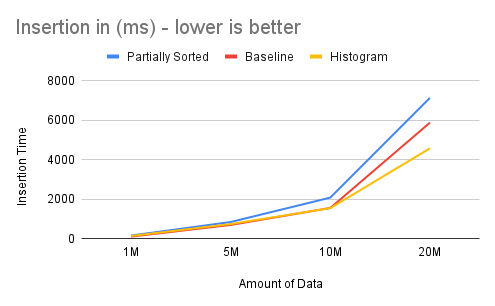
\includegraphics[width=100mm,scale=1]{Figures/InsertionResult.png}
    \caption{
     Results of Insertion Operation with Gaussian Distribution 
    }
    \label{fig:GraphInsertionResult}
\end{figure}

The empirical analysis we conducted, which is presented in Table \ref{tab:InsertionResult} and Figure \ref{fig:GraphInsertionResult}, revealed that gap optimization using the histogram is a superior algorithm to the baseline with \acrshort{fmcd} \cite{LIPP} and partially sorted gapped array algorithms when the data follows Gaussian Distribution. This was evident from the performance gains realized by the histogram-based algorithm, which was able to capture the distribution of the data and distribute gaps based on the data's distribution, thus performing better than the \acrshort{lipp} when newly inserted data followed the same distribution as the existing data.

Moreover, the histogram-based algorithm's performance superiority over the baseline algorithm was found to widen as the amount of data stored in the \learnindex tree increased, as depicted in Figure \ref{fig:GraphInsertionResult}. This can be attributed to the histogram's efficient distribution of gaps in the data based on its distribution, which enables it to maintain optimal performance even with larger data sets.

Conversely, the partially sorted gapped array algorithm performed the worst among the three algorithms. This was mainly due to its requirement to perform a sequential search within the gapped array to locate empty spaces before inserting new data. As a result, the partially sorted algorithm's performance deteriorated as the amount of data stored in the \learnindex tree increased, as illustrated in Figure \ref{fig:GraphInsertionResult}. With larger amounts of data, there were more conflicts, which caused the partially sorted \learnindex to conduct more sequential searches, resulting in inferior performance compared to the baseline and histogram gap optimization algorithms.


\paragraph{Lognormal Distribution}
\begin{table}
    \centering
    \begin{tabular}{ |p{2cm}|p{2cm}|p{2cm}|p{2cm}| } 
        
     \hline
     \multicolumn{4}{|c|}{Insertion Performance Result for Lognormal Distribution (in ms)} \\
     \hline
      Num Keys & Baseline (\acrshort{lipp})  & Partially Sorted & Histogram \\
     \hline
     \textbf{1M} & 127 & 156 & 199 \\
     \textbf{5M} & 1310 & 1593 & 1244 \\
     \textbf{10M} & 2593 & 3580 & 2443 \\
     \textbf{20M} & 5129 & 5930 & 4835 \\
     \hline
    
    \end{tabular}
     \caption{Insertion Results with Lognormal Distribution}
    \label{tab:InsertionResultLognormal}
\end{table}

Upon analyzing the results presented in Table \ref{tab:InsertionResultLognormal} and Figure \ref{fig:GraphInsertionResultLognormal}, we can conclude that the gap optimization using histogram algorithm still performs better than the baseline and partially sorted gapped array algorithms when using Log Normal Distribution. The results reveal that the histogram algorithm's superior performance is due to its ability to capture the distribution of the data and distribute gaps accordingly, thereby achieving better performance than the \acrshort{lipp} when the newly inserted data follows the same distribution as the existing data.

\begin{figure}
    \centering
    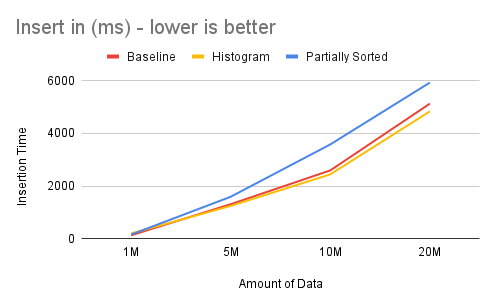
\includegraphics[width=100mm,scale=1]{Figures/InsertionResultLognormal.png}
    \caption{
     Results of Insertion Operation with Lognormal Distribution 
    }
    \label{fig:GraphInsertionResultLognormal}
\end{figure}
Similar to the findings with Gaussian Distribution, as the amount of data stored in the \learnindex tree increases, the performance gap between the histogram-based algorithm and the other two algorithms widens, as illustrated in Figure \ref{fig:GraphInsertionResultLognormal}. This can be attributed to the histogram algorithm's efficient distribution of gaps in the data, which enables it to maintain optimal performance even with larger data sets.

On the other hand, the partially sorted gapped array algorithm performed the worst among the three algorithms, as observed in the results presented in Figure \ref{fig:GraphInsertionResultLognormal}. The reason for this inferior performance can be attributed to the extra computations required to search for empty spaces after the predicted position. With larger amounts of data, the partially sorted algorithm's performance further deteriorates due to the increased amount of recursive rebuilding required when the spaces after the predicted position run out. Additionally, since each node contains more partially sorted items, each node takes longer to perform recursive rebuilding, leading to reduced performance as the amount of data increases.

The findings from our evaluation underscore the importance of considering the distribution of data when designing algorithms for processing and storing data. The results indicate that gap optimization using the histogram is a more efficient algorithm than the baseline and partially sorted gapped array algorithms, particularly when the newly inserted data follows the same distribution as the existing data. Leveraging techniques such as gap optimization using histograms can optimize performance and efficiency in data processing and storage.

\paragraph{Powerlaw Distribution}

\begin{figure}
    \centering
    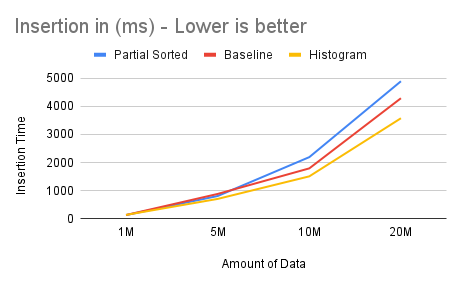
\includegraphics[width=100mm,scale=1]{Figures/InsertionResultPowerlaw.png}
    \caption{
     Results of Insertion Operation with Powerlaw Distribution 
    }
    \label{fig:GraphInsertionResultPowerlaw}
\end{figure}
It is important to note that power-law distribution is different from the other distributions tested in that it has a long tail, meaning that there are a few elements that frequently occur while most elements are rare. This property can make it more challenging to capture the distribution using a histogram-based approach accurately.

Additionally, the wider spread of the performance gap in Figure \ref{fig:GraphInsertionResultPowerlaw} compared to the other distributions indicates that the insertion operation is more unpredictable in power-law distributed data. This may be due to the highly skewed nature of the distribution, making it difficult to predict where new elements should be inserted accurately.

Despite these challenges, the histogram-based gap optimization approach still outperforms the baseline and partially sorted gapped array in power-law distribution. This suggests that the approach is still effective in capturing the distribution and distributing gaps accordingly, leading to better insertion performance.

The poor performance of the partially sorted gapped array in power-law distribution further supports the idea that this approach is unsuitable for indexing this data type. As the amount of partially sorted keys in each node increases with larger datasets, the amount of recursive rebuilding required also increases, leading to worse performance.


\paragraph{Real-World Dataset (Logitudes)}
\begin{figure}
    \centering
    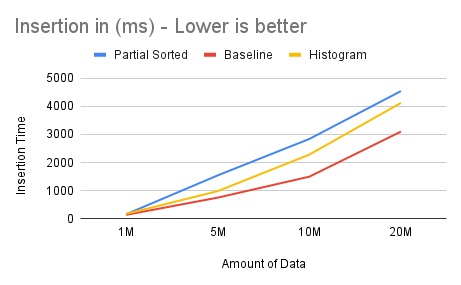
\includegraphics[width=100mm,scale=1]{Figures/InsertionResultLongitude.png}
    \caption{
     Results of Insertion Operation with Real-World Dataset 
    }
    \label{fig:GraphInsertionResultLongitude}
\end{figure}
To further analyze the result on a real-world dataset in Figure \ref{fig:GraphInsertionResultLongitude}, it is important to consider the nature of real-world data and how it can affect the performance of the algorithms. Real-world data is often diverse and can have a wide range of distributions, from uniform to skewed, and can also have varying degrees of correlation and clustering.

The baseline algorithm is able to perform better as it uses a \acrshort{fmcd} that distributes gaps and keys to optimize the linear regression model, and it does not require rebuilding during the insertion operation or does not have any assumption on the dataset. In other words, the baseline can be a good general purpose which performs well in any scenario. 

However, the histogram algorithm may not perform as well on real-world datasets as it does not account for the changing distribution of the data. The algorithm assumes that the data distribution is consistent and places gaps based on that assumption. This can lead to slower insertion times when the new data's distribution differs from the existing data.

Moreover, the partially sorted gapped array is not suitable for real-world datasets as it does not help the linear regression model improve its accuracy. Instead, it only delays the new node creation at a later stage to amortize the cost, which can be costly in terms of performance when there is a huge amount of data in the node.

The histogram algorithm is designed to work well when the distribution of the data is known, and it is able to adapt the gaps based on that distribution. But in real-world scenarios, where the distribution is not known or random, the baseline performs better as it is able to generalize to fit the randomness of the data. 

\subsubsection{Query}
To evaluate the performance of the query operation, we will test varying input sizes ranging from one million to twenty million, in order to determine which algorithms perform best in different scenarios and input sizes. Our tests will include both static (Gaussian, Lognormal, and Powerlaw) and dynamic (Longitudes) scenarios.

Testing static scenarios is important for query performance because it allows us to analyze the algorithms' behavior under specific data distributions. By using static datasets such as Gaussian, Lognormal and Powerlaw, we can evaluate how well the algorithms perform when the data follows a known distribution, and use this information to optimize the algorithm. For example, if an algorithm performs well on a Gaussian dataset, which is a commonly occurring distribution in real-world data, we can be confident that it will perform well on similar datasets in the future. This allows us to make more informed decisions when selecting which algorithms to use for specific tasks, and can help improve overall system performance.

Furthermore, testing static datasets allows us to measure the impact of the distribution on query performance, and identify any potential areas for optimization. This is particularly useful for algorithms that are designed to work with specific types of data distributions, such as the histogram-based algorithm that we tested earlier.

For each scenario, we will measure the query time taken by the baseline, histogram, and partially sorted algorithms. The results will be recorded and analyzed to determine which algorithm performs the best in each scenario.

This approach is necessary because different datasets may have different characteristics that affect the performance of the query operation. By testing different scenarios with varying input sizes, we can gain a better understanding of the strengths and weaknesses of each algorithm and determine which algorithm is the most suitable for a particular scenario.

Furthermore, by including both static and dynamic scenarios, we can compare the performance of the algorithms in scenarios where the data distribution is known beforehand and scenarios where the data distribution is constantly changing. This will provide valuable insights into the suitability of each algorithm in real-world scenarios where the data distribution is not known beforehand.

\paragraph{Gaussian Distribution}
The results of the experiment show that the performance of \learnindex algorithms varies significantly depending on the distribution of the input data. When it comes to query operations on the Gaussian Distribution, the histogram algorithm outperforms the other algorithms. This is because the histogram algorithm makes use of the gaps between keys that are specifically optimized for the given distribution. By doing so, it traverses lesser depth, which in turn improves the overall query performance.

On the other hand, the baseline algorithm performs relatively well compared to the partially sorted \learnindex algorithm. However, the baseline algorithm tries to generalize and perform well in most cases without taking advantage of the prior data distribution. This means its performance is less than the histogram algorithm in certain distribution types.

The partially sorted algorithm performs the worst of the other two algorithms in query operations. This is due to the extra computational overhead required when the keys are partially sorted. Even though the amount of conflicts is reduced with the partially sorted gapped array, the algorithm still spends a significant amount of time doing sequential searches due to potential miss predictions by the model and the partially sorted gapped array.

It is important to note that the above results were obtained in static scenarios, where the input data distribution remains constant. The histogram algorithm performed best in all static scenarios because it was specifically optimized for the given distribution. 

\paragraph{Lognormal Distribution}
The experiment was also conducted on a lognormal distribution dataset. Similar to the Gaussian distribution, the histogram algorithm outperformed the baseline \acrshort{lipp} and the partially sorted array in terms of query performance. The results shown in Figure 2 demonstrate that as the amount of data increases, the performance gap between the histogram and the baseline widens. This indicates that the histogram algorithm takes advantage of the data distribution and optimizes gaps in a way that allows the query to traverse fewer levels in the tree, leading to better performance.

On the other hand, the baseline algorithm still outperformed the partially sorted array even though the latter had a lower average tree depth. This is due to the extra computational overhead required for the $\epsilon$ linear search when there are a large number of partially sorted items in the tree. Despite having a lower average tree depth, the partially sorted array's slower search process prevented it from performing as well as the baseline in terms of query performance.

\paragraph{Powerlaw Distribution}
The study also evaluated the performance of the three data structures on Zipfian distribution. The results were similar to the other distributions, with the histogram performing the best and the partially sorted gapped array performing the worst.

The histogram data structure again outperformed the baseline and partially sorted \learnindex structures due to its optimization for the Zipfian distribution. The gaps in the histogram structure are also specifically designed to account for the high frequency of certain keys in the distribution, resulting in a lower average tree depth and improved query performance.

In contrast, the baseline \learnindex performed relatively well in querying Zipfian distribution, but still could not match the efficiency of the histogram. This is because the baseline tries to generalize and perform well in most cases, but does not take full advantage of the specific distribution characteristics.

The partially sorted gapped array again struggled with the Zipfian distribution, with the extra computational overhead of the $\epsilon$ linear search causing a significant performance gap from the other two structures. As with the other distributions, the partially sorted \learnindex performed better than the baseline \learnindex in terms of average tree depth. However, this improvement was outweighed by the increased search time from the linear search.

\paragraph{Real-World Dataset (Logitudes)}
Moving to a real-world dataset, the experimental result shows that the histogram performs on par with the baseline when it comes to range query. This indicates that both the baseline and histogram have a similar average tree depth which contributes to the similar query performance.

It is important to note that the query performance is heavily dependent on the height of the tree. If the tree height is greater, it leads to poor query performance. This can be attributed to the fact that a larger height would require the query algorithm to traverse through more levels of the tree, hence making the query more time-consuming.

However, when it comes to the partially sorted gapped array, the performance is still not up to the mark. Despite having a lower average tree depth compared to both baseline and histogram, the extra computation required for the linear search, after traversing the tree depth, hampers its overall query performance.


\subsubsection{Deletion}
In order to gain a deeper understanding of the performance of partially sorted and histograms compared to the baseline, we will conduct further experiments involving delete operations. This setup will be similar to the previous tests, with varying input sizes ranging from one to twenty million, using different distributions and a real-world dataset.

In the deletion operation, the performance is expected to be similar to that of the query operation, as the tree must be traversed to locate the keys before they can be deleted. This will provide us with additional insight into the efficiency of each algorithm and how they handle deletions.

These experiments will allow us to further analyze the performance of each algorithm in different scenarios, providing a more comprehensive understanding of their strengths and weaknesses.

\paragraph{Gaussian Distribution}
The results table showed that the histogram outperformed both the baseline and the partially sorted array in Gaussian distribution. This was due to the lesser average depth of the tree, which made traversing down the tree faster, allowing for faster deletions.

It was also observed that the baseline still performed better than the partially sorted, even though it had a higher average tree depth compared to the partially sorted array. This was due to the precise position of the keys from the model and not requiring an extra linear search like the partially sorted gapped array. 


\paragraph{Powerlaw Distribution}
For the Powerlaw Distribution, we use a similar strategy as other distributions where we bulk load the keys and then insert the same amount into the tree. The resulting Figure shows that the histogram still outperforms both baseline and partially sorted. The deletion works similarly to the query as it has to traverse down until it reaches a key before performing deletion which makes the deletion process bounded by the height of the tree. In this case, the reason why histogram achieve better performance is because it is able to make use of the gaps available in upper node and create lesser child node than the baseline. However partially sorted is slower even with similar tree depth is because it is bounded by the $\epsilon$ spaces and the height of the tree. The amount of time is mostly spent on the linear $\epsilon$ search which causes the gap in performance between the histogram and the partially sorted. 


Overall, the results showed that the histogram indexing algorithm was consistently the best performer in terms of query, insertion, and deletion operations across various distributions and real-world datasets. However, it is worth noting that the baseline algorithm also performed relatively well and could be considered as a viable alternative in scenarios where the data distribution is unknown. On the other hand, the partially sorted gapped array algorithm performed poorly and could be improved by reducing the number of partially sorted keys in the gapped array.


\paragraph{Real-World Dataset}
The real-world dataset serves as a more practical and relevant evaluation for these algorithms. The deletion operation is expected to have a similar performance to the query operation since both require traversing down the tree to locate the keys to be deleted or queried. As expected, the results show that the histogram and baseline perform similarly when deleting keys from the tree. This is due to their similar number of average tree height, which is a crucial factor that influences the query or deletion performance.

In contrast, the partially sorted gapped array performs worse than the histogram and baseline. Even though the partially sorted array has a lower average tree depth than the baseline, it requires an extra linear search after traversing down the tree to search for the predicted position of the key. This search is necessary because the keys could be located anywhere within a range of $x$ to $x + \epsilon$ around the predicted position. Consequently, the partially sorted array is bounded by the tree's height and the $\epsilon$ limit spaces after the predicted position. These factors contribute to its inferior performance compared to the histogram and baseline.


\subsubsection{Adjustment / Branch Pruning}
The \acrfull{lipp} algorithm is designed to optimize the performance of learned indexes by making adjustments to the tree's structure under specific conditions. These adjustments aim to reduce the tree's height, thereby reducing the time it takes to access and retrieve keys. During our testing of the learned indexes, we did not modify any of these conditions since they were already optimized for performance. However, we recognized that each of the algorithms (baseline, histogram, and partially sorted) has a unique implementation of these adjustments, which needed to be tested to determine the most effective implementation.

To test the effectiveness of these adjustments, we employed a rigorous testing strategy. We tested the algorithms on various data distributions, including Gaussian, Powerlaw, Lognormal, and Real-World datasets, and measured the execution time in milliseconds. By comparing the performance of the three algorithms, we aimed to identify which implementation of the adjustments was most effective.

From the result table, we observed that the histograms perform slower than the baseline on all test data. This is because the gap redistribution and retraining of the model required for the histogram adjustments result in an operating cost of $O(N\log N)$, which costs the same as the baseline $O(N\log N)$ \cite{LIPP}. The partially sorted algorithm also performed worse than the baseline and histogram algorithms. This can be attributed to the challenges associated with collecting partially sorted keys. Nevertheless, like the histogram algorithm, the partially sorted algorithm's adjustments were also dominated by the retraining of the model and the collection of keys.



\subsection{Memory Consumption}
In addition to measuring the execution time, it is also essential to analyze the memory consumption of each implementation. Memory consumption refers to the amount of memory that is required to perform each operation. Therefore, in this section, we will be using the same data set as before but measuring the memory consumption of each implementation.

Measuring memory consumption is crucial as it helps us determine the amount of memory resources required to run each algorithm effectively. By analyzing the memory consumption, we can optimize the algorithm to reduce its memory footprint, which is important in scenarios where memory is a scarce resource.

We will use the same testing strategy as before, running each algorithm on the same data set and measuring the memory consumption in bytes. By comparing the memory consumption of the three algorithms, we can determine which implementation is the most memory-efficient.

It is important to note that memory consumption is affected by various factors, such as the size of the data set, the structure of the data, and the algorithm's implementation. Therefore, the results obtained in this section will provide valuable insights into the memory consumption of each algorithm and help us optimize the algorithm for better performance.

\paragraph{Gaussian Distribution}

From the result Figure of the test on Gaussian Distribution, we can observe that the histogram performs best in terms of memory consumption, consuming the least compared to the partially sorted array and the baseline. The reason behind this is that the histogram maintains an array of frequencies in each node, allowing it to capture the distribution of the keys. As a result, it can predict the exact position of a key without having to perform a linear search when there is a miss prediction, leading to fewer conflicts and the creation of fewer child nodes, ultimately reducing memory consumption.

In contrast, the partially sorted array performs worse than the histogram, even though the main idea behind the partially sorted is to delay the creation of child nodes as much as possible. As the data set grows, there will be more partially sorted keys in each node, and when a conflict occurs and $\epsilon$ empty spaces run out, the algorithm still has to perform recursive rebuilding, creating numerous child nodes that consume memory. Therefore, the result is expected.

Moreover, the baseline implementation performs similarly to the partially sorted. The baseline algorithm aims to work well in most scenarios, which makes it perform worse when there are assumptions that can be taken advantage of. From the result Figure, we can see that the baseline creates more child nodes, which in turn consumes more memory than the partially sorted and histogram as the new nodes has to reserve some memory as \textsf{gaps} to be used for new keys.


\paragraph{Powerlaw Distribution}
Our memory consumption test on the Powerlaw Distribution shows a similar trend to that of the Gaussian Distribution. The histogram outperforms both the baseline and partially sorted array in memory consumption. The histogram consumes less memory, making it more efficient for use in a static scenario where the data distribution is known. It is able to create fewer child nodes, utilizing the \textsf{gaps} efficiently.

On the other hand, the partially sorted array delays the creation of new nodes to amortize the cost. However, as the amount of data increases, it will eventually have to spend a significant amount of time rebuilding nodes recursively. This means that the number of nodes that need to be rebuilt will continue to increase as more data is added to the \learnindex.

Similarly, the baseline performs similarly to the partially sorted array. It does not make any assumptions about the data distribution, unlike the histogram, which creates more child nodes than the baseline.

\paragraph{Lognormal Distribution}
The memory consumption test showed that the histogram outperformed the baseline and partially sorted \learnindex, which is consistent with the results from the Powerlaw Distribution. The histogram is able to maintain the distribution and gaps based on the data distribution, which allows it to have a lower average tree depth and consume less memory compared to the other two implementations.

On the other hand, the baseline only optimizes the keys based on the linear regression slope, which does not take into account the distribution of the data. As a result, it creates more child nodes and consumes more memory than the histogram. The partially sorted array delays the creation of new nodes to amortize the cost, but as the data becomes larger, it still needs to rebuild nodes recursively, resulting in more memory consumption.

Overall, the histogram is a more efficient implementation for static scenarios where the data distribution is known. Its ability to maintain gaps and distribution reduces the need for creating new child nodes and, thus, results in lower memory consumption.

\paragraph{Real-World Dataset}

However, for real-world scenarios where distribution is not known, the histogram performs worse than the baseline and is not able to capture the distribution of the data since the assumption is not valid for real-world data where distribution is known for newly insert keys. Since the histogram is not able to optimize based on the distribution, the histogram will cause more \conflict than the baseline which is expected and hence consume more memory. 

Similar to the histogram, the partially sorted method does not depend on any particular distribution. However, it defers resolving conflicts until all available empty spaces are filled, at which point it creates new child nodes. The results indicate that the partially sorted method performs slightly better than the histogram technique because it delays creating new nodes until a later stage. However, when there is a larger amount of data in the tree, the partially sorted method does consume more resources than the histogram. This is because it waits until the current node is completely filled before recursively rebuilding it, which uses up more memory.

When dealing with real-world datasets, it is advisable to use the baseline approach if memory consumption is a top priority. This method is highly adaptable and generally produces better outcomes than the histogram and partially sorted techniques. Nevertheless, if the data distribution is familiar, the histogram approach can be fine-tuned to better fit the data. 

\subsection{Number of New Node Creation / Tree depth}
In this section, we investigate the performance of three different \learnindex implementations, namely the histogram, partially sorted, and baseline, in terms of the number of new node creations or \conflict when using different datasets.

The number of \conflict is crucial in evaluating the performance of \learnindex algorithms, especially in dynamic scenarios, where the data distribution can change over time. For instance, when a new key is inserted into the tree, it may cause \conflict and result in new node creations to maintain the performance of the algorithm. Therefore, measuring the number of \conflict can provide insights into how well each \learnindex implementation adapts to changes in the data distribution.

We tested the three algorithms by performing bulk loading of one million to twenty million. After performing bulk loading we perform insertion for another one million to twenty million to test the trend and new node creation on different algorithms. Basically, we bulk load fifty percent of the keys in and insert another fifty percent later to perform experiment, which means that one million will have two million in the tree. 

\paragraph{Gaussian Distribution}
\begin{figure}
    \centering
    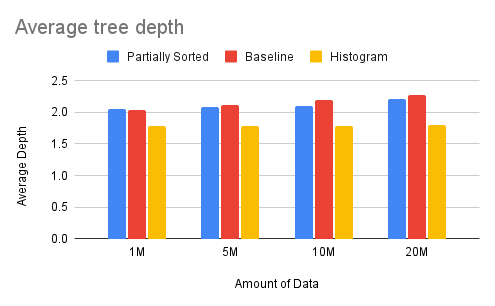
\includegraphics[width=100mm,scale=1]{Figures/AVGTD-Gau.png}
    \caption{
     Results of Average tree depth after a number of insertions (Gaussian)
    }
    \label{fig:AverageTreeDepthGau}
\end{figure}

From the results Figure \ref{fig:AverageTreeDepthGau}, we found that the histogram performs better on the average tree depth compared to the other two algorithms. Furthermore it has lesser \conflict number (new node creation) compared to partially sorted and baseline. This is because histogram is able to capture distributions of the data while partially sorted only delays \conflict until running out of space. This is inline with other experiments from previous sections. As lesser average tree depth improve operations performance as all of the operations are bounded by the height of the tree. For example, if we are able to reduce the depth of the tree, we will be able to reduce the time to perform read and write operations.

On the other hand, from result Figure \ref{fig:AverageTreeDepthGau}, the partially performs similarly to the baseline due, this is because the main idea of partially sorted is to store keys after the predicted position and reduce the number of new node creation. However, this is only delaying creating new node until later which will still be incured. This results inline with the operation experiments above as the amount of tree depth increase, the longer time it takes to perform read and write operation. Furthermore, the poor result on operations for partially sorted is due to the cost of recusively rebuilding the keys to be sorted.

In addition, the baseline performs worse than the histogram as the baseline implementation does not consider the data distribution, resulting in a higher number of average tree depth as it fails to optimize key positioning. From the results Figure \ref{fig:AverageTreeDepthGau}, can see that the baseline has higher average tree depth compared to histogram, which is inline with operations performance as histogram outperform the baseline in operations as well due to having lesser depth to traverse.



\paragraph{Powerlaw Distribution}
\begin{figure}
    \centering
    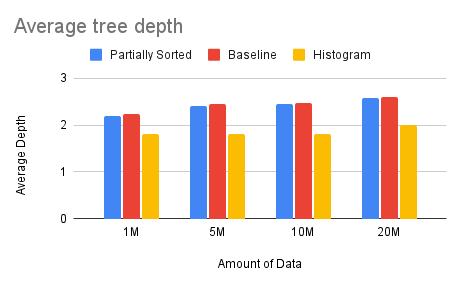
\includegraphics[width=100mm,scale=1]{Figures/AVGTD-Pow.png}
    \caption{
     Results of Average tree depth after a number of insertions (Powerlaw)
    }
    \label{fig:AverageTreeDepthPow}
\end{figure}
The result tested on Powerlaw distribution is not different from the Gaussian distribution (Figure \ref{fig:AverageTreeDepthPow}) where the histogram is able to outperforms both algorithm. This is because histogram can capture the distribution of the data and make use of the upper nodes gaps while the baseline just create new nodes whenever there is a \conflict and only wait until the next branch pruning (or adjustment) to occupy the upper nodes. 

Furthermore, partially sorted performs on par with the baseline as it only delays the new node creation until $\epsilon$ spaces runs out. From the result Figure \ref{fig:AverageTreeDepthPow}, we can see that the trend of average tree depth slowly increasing as more keys inserted in the tree. Even though the amount of data increase almost $10\times$, but the average tree depth does not increase much because of the branch pruning method that helps to reduce the amount of tree depth. However, we can see that the amount of average tree depth still increase for both partially sorted and baseline. While histogram is able to take advantage of the empty gaps in the upper node, which will create lesser new child node.


\paragraph{Lognormal Distribution}
\begin{figure}
    \centering
    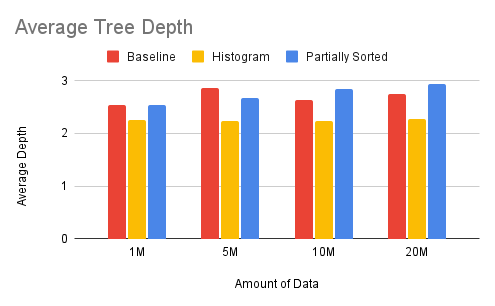
\includegraphics[width=100mm,scale=1]{Figures/AVGTD-Log.png}
    \caption{
     Results of Average tree depth after a number of insertions (Lognormal)
    }
    \label{fig:AverageTreeDepthLog}
\end{figure}
The result on Lognormal Distribution follows the same trend as previous distributions. However the main difference from the previous test is that the baseline seem to have lesser average tree depth from five million to ten million, this is because when it reaches a condition, the baseline will trigger branch pruning which reduces the tree depth. 

For histogram, we can see a similar trend where the histogram able to maintain the average tree height throughout the data increases. Which is inline with the result of insertion and search operations where it outperforms the baseline and partially sorted array. If it is able to make use of the upper nodes gaps, it will not need to wait until the branch pruning to make use of the available gaps in the upper nodes. 

\paragraph{Real-World Dataset}
\begin{figure}
    \centering
    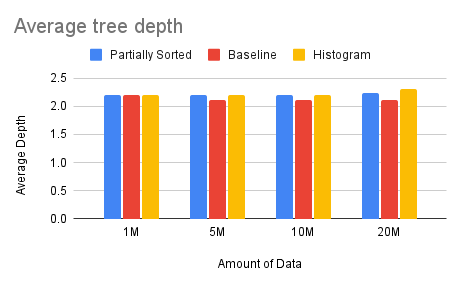
\includegraphics[width=100mm,scale=1]{Figures/AVGTD-Long.png}
    \caption{
     Results of Average tree depth after a number of insertions (Longitudes)
    }
    \label{fig:AverageTreeDepthLong}
\end{figure}
On the other hand, the results on dynamic scenario (Figure \ref{fig:AverageTreeDepthLong}) shows that the baseline outperforms histogram and the partially sorted. Based from the result Figure, we can see the baseline is able to make use of the gaps to insert and does not increase in the average depth while histogram does not perform when it comes to dynamic scenario as histogram can not capture the distribution which is crucial for histogram to work well. This results inline with the previous test on operations where baseline is able to out shine the histogram and partially sorted. This is because the search operation is only bounded by $O(h)$ where h is the height of the tree. This mean that reducing the amount of average tree depth will make the performance of the operations faster. 

Furthermore, the partially sorted perform similarly to both histogram and the baseline, as it make uses of the gaps by inserted keys after the predicted position which delays the new node creation, thus having lesser depth. However this does not inline with the operations performance, this is because the operation performance of the partially sorted is bounded not just by the height of the tree, but also $\epsilon$ spaces. Which is similar to the section on \nameref{partialsortedtheory} where we mentioned that the time complexity of the operations is $O(\epsilon + \log N)$


\subsection{Evaluation Summary}
In this section, we have compared the performance of three learned index algorithms: baseline, histogram, and partially sorted. Our testing showed that the histogram implementation outperforms the baseline in operations such as insertion, deletion, and query when the distribution is static, and new keys follow the same distribution. This is due to the histogram's ability to minimize the height of the tree by grouping keys with similar values into a single bin, leading to faster traversal times.

In addition, measuring the number of \conflict can provide valuable insights into the performance of \learnindex algorithms in dynamic scenarios. The histogram implementation performs the best in terms of the number of \conflict, followed by the partially sorted implementation, while the baseline implementation performs the worst on the static scenario. On the other hand, the baseline outperforms the histogram and the partially sorted on the dynamic scenario. If the data distribution is known, histogram seems to be a better fit to optimize the gaps while performing faster on operations. If the data distribution is not known, baseline seem to perform better as it generalize to fit in many scenarios. Furthermore, the partially sorted still need more experiments and improve as the searches is still bounded by the extra search spaces after the predicted position which makes it slower during read and write operations.

However, our testing also revealed that the histogram implementation needed further exploration to improve its performance in real-world scenarios where data is not static and can change over time. This is an area where the partially sorted algorithm falls short, as it requires extra computation that causes operations to slow down as the data increases in the tree.

In conclusion, the choice of the learned index algorithm depends on the characteristics of the dataset being indexed and the expected usage patterns. For static distributions, the histogram algorithm offers the best performance, while the partially sorted algorithm may be more suitable for dynamic data. Nonetheless, further research is needed to explore the potential of these algorithms in more diverse scenarios and to develop more advanced learned index structures that can handle more complex data distributions.

\section{Experimental Analysis}
In this section, we will perform in depth analysis on different parameters and the trade off between the two algorithm (Histogram and Partially Sorted). Different parameters will yield different result and base on the different dataset. The experiment method will be the same as the evaluation section where we will be using the same dataset. However, we will only limits to real-world dataset and one of the distribution due to the computation power in testing all of the distribution. We expect that the result will help gain more understanding on different parameters that the histogram and partially sorted introduced and its flaws and tradeoff.
\subsection{Histogram Bin} \label{Histogram Bin}
The choice of the bin size is important consideration when maintaining a histogram in each node. The bin size determines the number of bins used in the histogram and the range of values includes in each bin. The bin size should be chosen carefully to ensure that the resulting histogram accurately reflects the distribution of the data. 

If the bin size is too small, the histogram may not be able to capture the distribution of keys in the node and difficult to interpret. This is because each bin will contain only a small number of data points, and the resulting bar heights will be highly variable. Which makes it difficult to see the underlying pattern of the data.  

On the other hand, if the bin size is too large, the resulting of the histogram in each node may be too coarse and may not accurately capture the fine details of the distribution. This will result in important details to be missed out. 

In the Figure, we tested small static bin and the \acrshort{fdrule} to gain some insights on the data patterns and how bins affect the gaps optimization. Figure shows that the small bin size is able to capture the distribution and the underlying pattern as well as the \acrshort{fdrule}. The figure is taken from the histogram \acrshort{lipp} root node with a Gaussian distribution dataset on one million keys. we can see that the root node will contain the whole tree distribution. 

In this section, we will test the static bin size and Freedman-Diaconis rule to find the appropriate bin size and its tradeoff using the same dataset and setup as the previous section. However, in our calculation of the $bin\_index$, we have to find the $bin\_width$ which determines the range of keys that fall into this index. For example, if $bin\_width$ is equal to $1$,  that means the range of first index can be in the range of keys $0$ to $1$. With static bin size, we can calculate $bin\_width$ by $\frac{Key_{max} - Key_{min}}{bin\_size}$.

\paragraph{Gaussian Distribution} In this section, we aim to compare the performance of a static bin size of $10$ with the \acrshort{fdrule} when used in the histogram-based \learnindex algorithm on Gaussian Distribution. We carried out the same tests as in the previous section, but with the addition of comparing the performance of the different bin sizes.

From the resulting figure, we can observe that using a static bin size of $10$ does not perform well when there is a large amount of data in the tree. This is because the root node, which represents the entire distribution of the tree, does not capture the pattern well when the bin size is too small. As a result, the gap optimization in the tree performs poorly, causing the tree to grow deeper and impacting the read and write operations since they are bounded by $O(h)$ where $h$ is the height of the tree. Furthermore, we can also see that both the insertion and query operations perform poorly, due to the increasing height of the tree when the gap optimization does not work well. Additionally, the number of \conflict (or new nodes created) also increases, as the histogram-based \learnindex relies heavily on the histogram in each node to distribute gaps according to the frequencies.

In contrast, the \acrshort{fdrule} maintains a longer frequency (or bin) size, which consumes more memory compared to the static bin size. From the resulting figure, we can see that the \acrshort{fdrule} maintains $355$ bin sizes, while the static bin size only maintains $10$. This cost will be incurred when the adjustment triggers, and the algorithm has to rebuild the nodes. However, it offsets the operation cost, as the insertion operation has to traverse less depth compared to the static bin size. 

This makes the \acrshort{fdrule} performs well in term of representing the underlying patterns and able to make our gaps optimization works well on different distributions. It outperforms the static bin size when perform operations like the insertion, query and deletion due to the smaller depth that it has to traverse down.

\paragraph{Real-World Dataset} Real-world datasets can have a complex distribution, and unlike synthetic datasets with known distributions, it can be challenging to predict the distribution of new keys. Therefore, it is important to evaluate the performance of the \learnindex algorithms on real-world datasets to understand how they adapt to the underlying patterns.

Based on the results of our experiments on real-world datasets, we observed that the performance of the histogram \learnindex was poor compared to the baseline, as discussed in the previous section. However, in this experiment, we evaluated the performance of two different approaches, namely the static bin size and the \acrshort{fdrule}.

The results showed that both the static bin size and the \acrshort{fdrule} did not perform well when the distribution of new keys was unknown, as they were not able to capture the underlying patterns of the dataset. As a result, both approaches performed poorly on insertion and query operations compared to the baseline.

For memory consumption, the \acrshort{fdrule} approach performed worse than the static bin size. The \acrshort{fdrule} maintained more bin sizes, while not performing better on read and write operations. The static bin size approach, on the other hand, required less memory as it only needed to maintain a fixed number of bin sizes in each node.

Therefore, based on our experiments on one million real-world keys, the static bin size approach is a better solution when the distribution of new keys is unknown. This is because the \acrshort{fdrule} does not perform better than the static bin size on read and write operations while consuming more memory to maintain the frequencies of keys in each node. The static bin size approach only needs to maintain a fixed number of bin sizes in each node, and it performs better than the \acrshort{fdrule} when the distribution of new keys is unknown.


\paragraph{Summary}

In summary, the choice between the static bin size and the \acrshort{fdrule} depends on the trade-off between memory consumption and performance. When memory is not a concern, the \acrshort{fdrule} is the better option as it can optimize gaps based on the underlying data distribution and improve the read and write operations. The \acrshort{fdrule} maintains more bins compared to the static bin size, resulting in higher memory consumption. However, this cost is offset by the performance improvement, especially when the system is dealing with frequent query and insertion operations.

On the other hand, if the system is memory-constrained, the static bin size is the better option. The engineer can fine-tune the number of bins based on the data distribution, reducing the memory consumption while still maintaining acceptable performance. However, this approach requires a deeper understanding of the data distribution and the impact of different bin sizes on the \learnindex performance.



\subsection{Partially Sorted $\epsilon$ Spaces}
The $\epsilon$ spaces are a crucial factor in determining the performance of \learnindex, as it influences the traversal of the tree and the operation's runtime complexity. The $\epsilon$ parameter determines the number of gaps to search for in the gapped array when the predicted position is not empty. As all the operations are bounded by the $\epsilon$ spaces, the number of $\epsilon$ sets affects the search performance.

To determine the impact of the $\epsilon$ parameter on the search operation, we conducted experiments on different parameter values, namely $1$, $5$, and $10$, using the same datasets as in the previous section, i.e., Gaussian and Real-World datasets. We evaluated the performance of the insertion, query, and deletion operations using these different parameter values.

The $\epsilon$ parameter has a significant impact on the search operation's performance. In general, a larger value of $\epsilon$ will result in a higher number of gaps to search for, making the search operation more efficient as query has to traverse down lesser depth due to smaller tree heigit. However, a larger value of $\epsilon$ also increases the memory overhead of the index, as more gaps need to be stored. 

On the other hand, a smaller value of $\epsilon$ will result in fewer gaps to search for, making the new node creation higher which will make the search operation in efficient. However, a smaller value of $\epsilon$ also reduces the number of search after the non-empty spaces.


\paragraph{Gaussian Distribution}In the case of the Gaussian Distribution, we inserted keys with the same distribution as the keys that were already present in the tree. However, we do not expect the partially sorted data structure to perform well on this distribution as it only delays the slow operation of new node creation until the gaps are full. The results from the Insertion operation Figure show that the trend of results changes as the number of $\epsilon$ decreases, indicating that the insertion operation becomes faster as the number of searches it has to perform decreases. However, if we look at the graph, we can see that the number of new node creations increases as the number of $\epsilon$ decreases.

In addition, querying keys in the partially sorted data structure has the same performance trend as the insertion operation. This is because they both have the same time complexity, which is $O(\epsilon+\log N)$. This complexity is bounded by the search after the predicted position. Based on our results, it seems that the time to search a key is mostly dominated by the $\epsilon$ linear search as the trend of the search performance seem to decreases while the $\epsilon$ also decreases. However the number of nodes creation inversely related to the $\epsilon$ because the smaller the $\epsilon$, the number of lesser gaps to delay new node creation. 

The importance of the $\epsilon$ parameter in the partially sorted data structure is enormous, as all operations are mostly bounded by the traversals down the tree height and the $\epsilon$ spaces (or $O(\epsilon+\log N)$). The $\epsilon$ parameter determines the number of gaps in the gapped array to search for when the predicted position is not empty. Since all operations are bounded by the $\epsilon$ spaces, the number of $\epsilon$ sets will affect the search performance. 

Furthermore, its effectiveness heavily depends on the choice of the parameter $\epsilon$, which determines the number of gaps to search for when the predicted position of a key is not empty. This choice can require significant engineering effort, and even with a well-chosen $\epsilon$, partially sorted may not outperform other data structures.

In comparison to baseline and histogram data structures, which are only bounded by the height of the tree, partially sorted suffers from the need to delay the creation of new nodes until gaps are filled. This means that partially sorted does not assume any underlying pattern in the data distribution, but instead aims to optimize search and insertion by using the gaps as a buffer.

\paragraph{Real-World Dataset} When applied to real-world datasets, the partially sorted algorithm demonstrates a similar performance trend to that seen in static scenarios. When compared to other algorithms such as baseline and histogram, the partially sorted algorithm may not always be the most efficient. Nevertheless, this section of our study focuses on comparing the performance of different partially sorted parameter settings.

The results presented in the figure clearly show that partially sorted with $\epsilon = 1$ performs best in operations such as insertion, deletion, and query. This is because this setting only requires one space search after the predicted position, which can significantly improve the algorithm's performance. Since the time complexity of the algorithm is bounded by $\epsilon+\log N$, a lower value of $\epsilon$ leads to faster operations.

However, when $\epsilon$ is decreased, the memory consumption of the algorithm increases. This is in line with our expectations, as reducing the number of spaces only delays the new node creation process for one conflict. As a result, there are more child nodes with lower $\epsilon$ values, leading to increased memory usage.

In summary, the value of $\epsilon$ in partially sorted refers to the number of limits that the algorithm can locate, which only delays the new node creation process. This algorithm does not take advantage of the underlying pattern of the keys, making its results similar for both real-world datasets and static scenarios. Therefore, selecting the optimal value of $\epsilon$ for a given dataset is critical to achieving the best performance of the partially sorted algorithm.

\subsection{Tradeoff}
Tradeoff is a crucial aspect of designing a \learnindex structure as it involves balancing size, accuracy, and efficiency. However, the accuracy can be eliminated by introducing new node creation in \acrshort{lipp} algorithm \cite{LIPP}, which leads to exact predictions but increases the size of the structure as a new node is created each time the predicted location is already occupied. In contrast, the partially sorted algorithm introduces the accuracy tradeoff in terms of $\epsilon$ which determines the number of keys that can be located in the structure.

In this section, we will compare the tradeoffs between Histogram and Partially Sorted parameters using the results obtained in the previous section. Although the Histogram algorithm does not require an accuracy tradeoff as the predicted position is exact and the time complexity is bounded by the height of the tree. In contrast, Partially Sorted provides a balance between accuracy, size and efficiency tradeoffs, but it may not perform as efficiently as Histogram or other algorithms in certain scenarios. Therefore, it is important to consider the specific use case and requirements when deciding which algorithm to use.

\paragraph{Histogram}
In the previous section on \nameref{Histogram Bin}, we compared the performance of different bin sizes in a static scenario with a Gaussian Distribution. We found that the histogram outperformed the baseline and partially sorted algorithms. However, we also found that the choice of bin size plays a significant role in the accuracy and efficiency of the algorithm. If the bin size is too small, the histogram will not be able to capture the distribution of keys in the tree, resulting in poor accuracy. On the other hand, if the bin size is too large, the distribution will be too coarse, also resulting in poor accuracy. Hence, there is a tradeoff between bin size and the visibility of underlying patterns.

In terms of node size and memory consumption, a static bin size is the best option. However, this approach sacrifices the efficiency of the operations such as insertion, deletion, and query. This is because each node may have a different distribution, and a static bin size will not be good enough for all of them. Consequently, more conflicts will occur, and the \learnindex will have to create more new nodes, making operations less efficient. Tuning for a good enough bin size becomes challenging as the tree grows larger, and each node has its own distribution, which cannot use a "one size fits all" approach.

In contrast, \acrshort{fdrule} helps determine the bin size based on the keys in each node. This approach decides the bin size in each node such that it is good enough to distribute gaps based on the frequencies array. However, the tradeoff for this implementation is that it will consume more memory in each node as it has to maintain the array of frequencies. Due to variable bin size, the accuracy of distributing gaps increases, which decreases the number of conflicts. Thus, operations performance increases, as seen from the previous section.

From our experiment, we conclude that using \acrshort{fdrule} is the best approach as it determines a good enough bin size for each node, resulting in higher accuracy and fewer conflicts. However, controlling the amount of memory consumption can be challenging. It is essential to balance memory consumption and performance to achieve the optimal solution. We argue that optimizing operations performance is the best approach since insertion and query operations occur frequently in real-world systems where users have to keep the data updated. Thus, the efficiency of these operations plays a critical role in the overall system performance.


\paragraph{Partially Sorted} 
In this section, we discuss the tradeoff between size, efficiency and accuracy in the context of \learnindex with partially sorted arrays. Unlike histogram bins, partially sorted arrays use the concept of partial limit spaces or $\epsilon$ to delay the slow new node creation by storing it a few $\epsilon$ spaces after predicted position. $\epsilon$ defines the number of spaces that the algorithm has to search for after the predicted position. Therefore, the operation performance like insertion is bounded by $\epsilon + \log N$, where $N$ is the number of keys in the node. In this section, we will be experimenting with different values of $\epsilon$ to determine the tradeoff between size, efficiency, and accuracy.

From the experimental results in Figure, we observe that the performance of partially sorted arrays improves as $\epsilon$ increases. This is consistent with the theoretical analysis that suggests that the performance is not only bounded by $\log N$, but also by the $\epsilon$ spaces that the algorithm has to search. On the other hand, partially sorted arrays do not need to store any extra information like histogram bins, where a frequency array is maintained for each node. To determine if a key is partially sorted or not, we simply use the model to predict the position of the key and compare it with the current position. If the predicted position is different from the current position, then it is a partially sorted key.

In terms of operation performance, we observe that insertion is the most impacted operation by the choice of $\epsilon$. The reason for this is the recursive rebuild operation that is triggered when the $\epsilon$ spaces are exhausted. In particular, when the number of partially sorted keys in the node is high, the number of recursive rebuild operations required also increases, thereby reducing the efficiency of the insertion operation.

Based on the experimental results, we can conclude that $\epsilon = 1$ offers the best tradeoff between size and performance in terms of operations like insertion. However, as $\epsilon$ increases, the performance of the partially sorted array also improves, but at the cost of increased memory consumption due to the need to store more partially sorted keys. For example, when $\epsilon = 5$, the performance of insertion is significantly worse than when $\epsilon = 1$ due to the increased number of recursive rebuild operations required to insert a new key.

In conclusion, the choice of $\epsilon$ in partially sorted arrays determines the tradeoff between size, efficiency, and accuracy. While a smaller value of $\epsilon$ improves the performance of operations like insertion, a larger value of $\epsilon$ improves the overall performance of the algorithm at the cost of increased memory consumption. Therefore, it is important to strike a balance between these tradeoffs when implementing \learnindex with partially sorted arrays.

\subsection{Maximum Gaps} In this section, we will delve deeper into an experiment to explore how different gaps distributions affect the performance and memory consumption of Histograms. This experiment is essential because the number of gaps that we distribute will affect the overall usage of memory as the gaps have to be reserved for key insertion.

In this experiment, we will test different datasets, such as Gaussian distributions and real-world datasets, to observe the changing trends and the trade-offs on different settings of gap distribution. We will also test different gap distributions such as $2\times$, $2.5\times$, and $3\times$. The $2\times$ refers to double the size of keys currently collected in the adjustments. The adjustment or branch pruning is only done based on the mentioned condition. For example, if we collected keys of $[1,2,3]$, the size of the expanded array will be $2\times 3$ which is $6$ so there will be $3$ keys and $3$ gaps. However, for $2.5\times$ the size, if the outcome of multiplication contains a decimal, we will round it up and place the leftover gaps at the end of the array.

In the experiment on the Gaussian distribution, the results show that distributing gaps $3\times$ the size of keys collected performs best in terms of new node creation, as it has more gaps to locate keys in, which will reduce the number of child nodes. This setting can also increase the operation performance like insertion, as it traverses to a lesser depth than the $2\times$ and $2.5\times$ settings.

However, the memory consumption is affected by the increasing number of gaps, which is a tradeoff between size and efficiency. From the memory consumption figure, we can see that the amount of memory consumed by $3\times$ increases from $2\times$ and $2.5\times$.

If the operation performance is the main concern, distributing more gaps can help reduce the number of new node creations while consuming more memory, as the gaps must be reserved for new keys, which is in line with the theoretical analysis that the performance is bounded by the height of the tree ($O(\log N)$). That means if we can reduce the height of the tree, we will gain performance in operations like insertion, deletion, and query. However, if memory is the primary concern, distributing more gaps will consume more memory.

From our testing, it seems that the $2\times$ setting is the best tradeoff between operation performance and memory consumption, as the operation performance trend does not increase as much as the memory consumption. From the figure, we can see that the $3\times$ gaps distribution increases memory consumption much more than it increases operation performance. Which makes $2\times$ the best tradeoff in performance and size.

For the real-world dataset, a similar trend appears that the maximum number of gaps to distribute will have more gaps for the model to insert new keys into. Based on the figure, we can see that the histogram performs better in terms of operation performance as it reduces the number of new child nodes because it has more gaps for the machine learn index to place new keys in. When there are fewer child nodes, the operation performance increases, which is in line with the theoretical analysis, where the operation performance for histograms is bounded by how much the height of the tree grows.

However, expanding more gaps $3\times$ consumes extra memory (figure) as the gaps have to be reserved for new keys, which will consume memory. Furthermore, we can see from the figure that the amount of memory consumption increases when we distribute more gaps. However, the gain in operation performance is not significant and does not outweigh the fact that memory consumption trend increases higher than the operation performance. Which makes $2\times$ the number of collected keys the best tradeoff between operation performance and memory consumption in real-world datasets.

In conclusion, distributing more gaps can help reduce the number of new node creations and increase operation performance, but at the expense of memory consumption. The optimal gap distribution is a tradeoff between operation performance and memory consumption, with $2\times$ being the best setting for most scenarios.

\subsection{Scalability }In this section, we will delve into the scalability of two indexing algorithms, namely the histogram and partially sorted index, by analyzing their performance on datasets of varying sizes. We will be using the same datasets as the previous section, but this time with an increase in the number of insertions. We will test on datasets with sizes of $10M$, $20M$, and $50M$ and also perform tests on both Gaussian distribution and real-world datasets.

The performance of an indexing algorithm is crucial when dealing with large datasets as it determines the speed of insertion, query, and building. A good indexing algorithm should be able to handle large datasets efficiently, without sacrificing performance. The scalability of an indexing algorithm is, therefore, an important factor to consider when selecting an indexing algorithm.

To test the scalability of the histogram and partially sorted index, we will perform insertion, query, and building operations on datasets of varying sizes. We will start by inserting $10M$ keys into both indexing algorithms and measure their performance. We will then repeat the process with datasets of sizes $20M$ and $50M$.

Additionally, we will test the scalability of the algorithms on two different types of datasets. The first type is the Gaussian distribution, which is a well-known distribution often used to test algorithms. The second type is a real-world dataset, which is more complex and closer to the kind of data an algorithm would encounter in a practical scenario.

When it comes to query performance on Gaussian Distribution, the histogram has a clear advantage over the partially sorted approach. This is because the histogram, as an extension of \acrshort{lipp}, only needs to traverse down the tree depth to locate the keys, while partially sorted requires a search just like other \learnindex algorithms. In our tests using the Gaussian Distribution dataset, we found that query time increases as the amount of data increases and the tree height grows larger for the histogram. This is consistent with the theoretical prediction that query time is bounded by the height of the tree.

On the other hand, the partially sorted approach showed the highest growth rate compared to the baseline and histogram. This is because the algorithm has to perform a local search for $\epsilon$ after traversing down the tree depth. As per the theoretical analysis, query time is bounded by $O(\epsilon + \log N)$, which makes the partially sorted approach not scalable as the amount of data increases. When there are many partially sorted keys within each node, the performance of the partially sorted approach is affected, which makes it slower than other \learnindex algorithms.

Insertion time shows a similar trend to query performance, where the histogram outperforms the partially sorted approach as the data size increases. When the data size is small, the partially sorted approach tends to outperform the histogram because it delays new node creation, while the histogram creates a new node only when there is a conflict. However, when the amount of data increases, and more partially sorted keys are inserted into each node, the performance of the partially sorted approach worsens as it has to perform recursive rebuilding. This slows down the insertion performance compared to the histogram since the recursive rebuilding cost is $O(\frac{N}{2})$, where $N$ is the number of keys in the node.

When it comes to query and insertion performance in real-world datasets, we have seen that the histogram approach may not be as effective as it is in the Gaussian distribution. However, the general trend of histogram outperforming partially sorted is still observed. This is because, in histogram, we only need to traverse down the tree depth to locate the keys, whereas in partially sorted, we need to perform local search similar to \acrshort{alex}\cite{ALEX}. As the amount of data increases, the number of partially sorted keys also increases, which in turn increases the depth of the tree. Therefore, we observe a linear increase in partially sorted performance with increasing data size. However, histogram can still create new nodes and increase the tree depth without the need for local search, making it more scalable than the partially sorted approach.

Furthermore, the trend in insertion performance is also similar to that of query performance. When the amount of data is small, partially sorted tends to outperform the histogram as it delays the creation of new nodes. However, as more data is inserted into the tree, the number of partially sorted keys in each node increases, which triggers recursive rebuilding that can slow down the insertion performance. In contrast, the histogram approach still outperforms partially sorted because it only needs to traverse down the tree depth and create new nodes when there is a conflict, without the need for local search. This makes the insertion operation faster in histogram than in partially sorted.

In summary, the histogram approach is more scalable than the partially sorted approach for both query and insertion operations, especially when dealing with large amounts of data, as histogram does not require any extra searches after traversing down the tree compared to partially sorted keys.


\section{Conclusion}
\subsection{Contribution}
In summary, this thesis proposes two new strategies to optimize \learnindex: the Histogram and Partially Sorted Insertion Strategy. The Histogram method aims to capture the distribution and pattern of the data by maintaining a frequency array in each node. The gaps are distributed where they are needed the most, based on the data distribution, which helps to minimize the number of child nodes and improve the operation performance.

The Partially Sorted Insertion Strategy works by delaying the creation of new nodes until the amount of $\epsilon$ is full. This approach helps to reduce the number of child nodes created and optimize the memory consumption of the \learnindex.

To evaluate the performance of the proposed methods, we conducted experiments on various parameters such as memory consumption, the number of child nodes, and operation performance, and compared the results with the baseline \acrshort{lipp} method. The experiments show that the Histogram outperform the baseline \acrshort{lipp} method and partially sorted insertion strategy in terms of memory consumption and operation performance. We hope that our algorithms complement the existing studies on the dynamic learned index.

\subsection{Limitation}
Despite the advantages of the histogram and partially sorted, there are still some limitations to consider. One limitation of the histogram is its performance on real-world datasets, where it does not capture the distribution as well as the raw \acrshort{lipp}. This is because histogram creates child nodes whenever there is a conflict, which can significantly affect the operation performance. In contrast, \acrshort{lipp} creates less child nodes and performs better in capturing the distribution of real-world datasets.

Another limitation of partially sorted is that it still does not perform as well as \acrshort{lipp} and histogram due to the extra local search that it has to perform. While partially sorted delays new node creation, it requires additional operations to maintain its partially sorted property, making it slower than \acrshort{lipp} and histogram. Additionally, our research mainly focuses on the efficiency and memory consumption of these \learnindex structures, without delving into their model accuracy. Future research could explore the triangular tradeoff between model accuracy, size, and efficiency in partially sorted.

In summary, while histogram and partially sorted have advantages over other \learnindex structures, they still have limitations that need to be considered. Understanding these limitations can help researchers and practitioners choose the best \learnindex structure for their specific use case.

\subsection{Future Work}
In this section, we put forward some potential avenues for future research that could enhance both the histogram and partially sorted array, with the goal of further improving the performance of the \learnindex. By doing so, we hope to provide guidance for future studies that can build upon our findings and push the limits of what is possible with the \learnindex.
\paragraph{Histogram}
 one limitation of the histogram is that it assumes the dataset has a fixed and known distribution. In practice, this is often not the case, as real-world datasets may have outliers and do not follow a known distribution. This limitation can affect the accuracy of the histogram, leading to suboptimal query processing performance. Therefore, there is a need to improve the histogram to support dynamic datasets with changing distributions.

To address this limitation, one possible improvement is to add a mechanism to the histogram that triggers the rebuilding process when certain conditions are met. This mechanism can be based on statistical measures such as the variance of the data or the deviation from the expected distribution. When the histogram detects that the data's distribution has significantly changed, it can rebuild the histogram with the new distribution parameters.

This improvement can benefit many database systems that rely on histograms for query processing. By adapting to the changing distribution of the data, the histogram can provide more accurate estimates of the frequency distribution, leading to better query performance.


\paragraph{Partially Sorted}
One possible improvement for the current work of the Partially Sorted Insertion Strategy is to introduce a parameter to keep track of the number of partially sorted keys in each node. With this parameter, we can set a threshold for the percentage of partially sorted keys in each node. For example, if the percentage of partially sorted keys in a node exceeds $50\%$ of the node size, then the node will perform a recursive rebuild. This threshold can be adjusted based on the specific dataset and the performance requirements of the application.

By introducing this improvement, we can reduce the number of partially sorted keys that have to be collected and rebuilt during insertion, which can improve the overall insertion performance of the partially sorted array. Moreover, it can also prevent the accumulation of too many partially sorted keys in a node, which can cause the tree to grow too deep and negatively affect the query performance.
\addcontentsline{toc}{section}{Bibliography}
\bibliographystyle{acm}
\bibliography{bib}
\end{document}
